\documentclass[14pt]{beamer}
\usepackage[T2A]{fontenc}
\usepackage[utf8]{inputenc}
\usepackage[english]{babel}
\usepackage{amssymb,amsfonts,amsmath,mathtext}
\usepackage{cite,enumerate,float,indentfirst}

\usepackage{multicol}
\usepackage{listings}

\graphicspath{{images/}}

\usetheme{Pittsburgh}
\usecolortheme{whale}

\setlength{\columnseprule}{1pt}
\def\columnseprulecolor{\color{blue}}

\setbeamercolor{footline}{fg=blue}
\setbeamertemplate{footline}{
  \leavevmode%
  \hbox{%
  \begin{beamercolorbox}[wd=.333333\paperwidth,ht=2.25ex,dp=1ex,center]{}%
    Boris Kudryashov, ITMO University
  \end{beamercolorbox}%
  \begin{beamercolorbox}[wd=.333333\paperwidth,ht=2.25ex,dp=1ex,center]{}%
    St. Petersburg, 2016
  \end{beamercolorbox}%
  \begin{beamercolorbox}[wd=.333333\paperwidth,ht=2.25ex,dp=1ex,right]{}%
  Page \insertframenumber{} of \inserttotalframenumber \hspace*{2ex}
  \end{beamercolorbox}}%
  \vskip0pt%
}

\newcommand{\itemi}{\item[\checkmark]}

\title{\small{Information Theory. 2nd Chapter Problems}}
\author{\huge{
Boris Kudryashov \\
\vspace{30pt}
ITMO University
}}


\begin{document}

\maketitle

\begin{frame}
\frametitle{Problems}
\begin{enumerate}
  \item[1] Construct a  Huffman code for the source with probability distribution:
  
  $(0,3, 0,25, 0,15, 0,1, 0,1, 0,05, 0,05)$
  
  Compare the average codeword length with the entropy.
  \pause \item[2] Consider Discrete Memoryless Source (DMS) $X = \{a, b, c\}$ with probability distribution: 
    \begin{enumerate}
    \item
    $p\left( a \right) = 1/2,p\left( b\right) = 1/4,p\left(c\right)=1/4;$
    \item
    $p\left( a \right) = p\left( b \right) = p\left( c \right) = 1 / 3.$
    \end{enumerate}
  Find Huffman codes for $X$, $X^{2}$, $X^{3}$. Compare code rate with the entropy of the source.
\end{enumerate}
\end{frame}


\begin{frame}
\frametitle{Problems}
\begin{enumerate}

  \item[3] Analyse behaviour of the Huffman code rate as a function of length $n$ of encoded blocks for the Binary Memoryless Source (BMS) with probability of $1$ equal to 0.1.
 
\end{enumerate}
\end{frame}


\begin{frame}
\frametitle{Problems}
\begin{enumerate}

  \item[4] \emph{Optimal coding for uniform distributions} 
  Find a Huffman code for source, which chooses letters from alphabet of size $M$ with uniform distribution. Calculate the average length of codewords and redundancy as a function of $M$, derive upper and lower bounds of redundancy.
  
  \end{enumerate}
\end{frame}


\begin{frame}
\frametitle{Problems}
\begin{enumerate}
   
  \item[4 (hint)] 
  \small{ \emph{Intermediate steps} Huffman code for this source contains $D=2\cdot 2^{\lfloor \log M \rfloor} - M$ words of length 
$\lfloor \log M \rfloor$ and  $M-D$ words of length $\lfloor \log M
\rfloor+1$. Average length of codewords and redundancy are equal to 
\[
\bar l =\lfloor \log M \rfloor+2-\frac{2}{M}%
2^{\lfloor \log M \rfloor},
\]
\[
r=\bar l - \log M= 2-d-2\cdot 2^{-d},
\]
where $d=\log M - \lfloor \log M \rfloor$, $d\in[0,1)$.
Differentiation with respect to $d$ shows, that maximum of redundancy is achieved when $d=1-\log\log e$ and is equal to $1+\log\log e - \log e
\approx 0,0861$.
  }
\end{enumerate}
\end{frame}


\begin{frame}
\frametitle{Problems}
\begin{enumerate}
  
  \item[5] 
  \small{ Consider Markov chain with the probability transition matrix:
\[
P = \left[ {{\begin{array}{*{20}c}
 0 \hfill & {1 / 2} \hfill & {1 / 2} \hfill \\
 {1 / 2} \hfill & {1 / 4} \hfill & {1 / 4} \hfill \\
 {1 / 4} \hfill & {1 / 2} \hfill & {1 / 4} \hfill \\
\end{array} }} \right].
\]
  Calculate $H\left( X \right)$, $H_n \left( X \right)$,  $n = 1,2,...$, $H\left( {X / X^n} \right)$, $n = 1,2,...$, assuming that the initial distribution on letters is the stationary distribution.
  Find code rate for coding ensembles $X$ and $X^2$ using Huffman coding. Suggest such a method for encoding, that code rate is equal to the information rate of the source. 
  }
\end{enumerate}
\end{frame}


\begin{frame}
\frametitle{Problems}
\begin{enumerate}
  \item[6] \small{  \emph{Non-uniform series-length coding} 
  Sequence at the output of binary source is uniquely represented in the form of concatenation of subsequences $1,01,...,0^{L - 1}1,0^L$ for some integer R. 
  Then a Huffman code is used for encoding indices of subsequences from this set.
  For a BMS with probability of $1$ equal to $p$=0,1, analyse the dependence between code rate and the value $L$ . 
  
  Code rate in this case is a value $R = \bar{n} / \tau ,$ where \textit{$\tau $} -- average length of sequence to be encoded; $\bar {n}$ -- average length of codewords.
}
\end{enumerate}
\end{frame}


\begin{frame}
\frametitle{Problems}
\begin{enumerate}
  \item[7] 
  \footnotesize { \emph{Variable-to-Variable  (VV) codiing. Tunstall code.}
  
  Recall that the redundancy of the Huffman code is determined by the maximum probability of letters. 
  
  Let $X={p(x)}$ and $x_0\in X$  is a most probable letter. Introduce a new ensemle $X_1$, which consists of all letters from $X\setminus{x_0}$ and of all pairs $(x_0,x)$, $x\in X$. Probabilities of pairs of letters are calculated like products of probabilities of corresponding letters. 
  Such extension of the alphabet can be continued, and on each next step, the maximal probability of letters of the extended alphabet becomes smaller. Thus the redundancy of code applied to the extended alphabet also becomes smaller.

  Compare this way of encoding to series-length coding, considered in previous problem for a random binary ensemble 
 
}
\end{enumerate}
\end{frame}


\begin{frame}
\frametitle{Problems}
\begin{enumerate}
\item[8] Construct Shannon code of the source from task 1. Compare its average length with the average length of Huffman code codewords and with entropy of the source.

\pause \item[9] Construct Gilbert-Moore code of the source from task 1. Compare its average length with the average length of Huffman code codewords and with entropy of the source.

\end{enumerate}
\end{frame}


\begin{frame}
\frametitle{Problems}
\begin{enumerate}

 \item[10] Use arithmetic coding to encode the sequence $01001$ from the BMS with probability of $1$ is $0.4$
 Compare the length of code sequence with the amount of information of the sequence. 
 Compare the length of code sequence with the total length of code sequence assuming independent encoding of characters with Shannon code.
 
\pause \item[11] Explain, why completing step of encoding in the program (p. 87, pic. 2.16 in the book) is equivalent to conversion of the codeword of Shannon code to codeword Gilbert-Moore code.

\end{enumerate}
\end{frame}


\begin{frame}
\frametitle{Problems}
\begin{enumerate}


 \item[12] What changes should be done in the algorithms and programs of arithmetic coding and decoding, to apply them to source, described by Markov chain.
 

\pause \item[13]  In programs at the pictures (p. 87, pic. 2.16) and (p. 88, pic. 2.17) in the book appear division operations which did not exist in algorithms of arithmetic coding and decoding. Why? Is it possible to avoid divisions here?


\end{enumerate}
\end{frame}


\begin{frame}[fragile]
\frametitle{Problems}


  \begin{multicols}{2}
  \includegraphics[width=0.28\textwidth]{fig_ar_encoder.eps}
  
  \columnbreak
  
  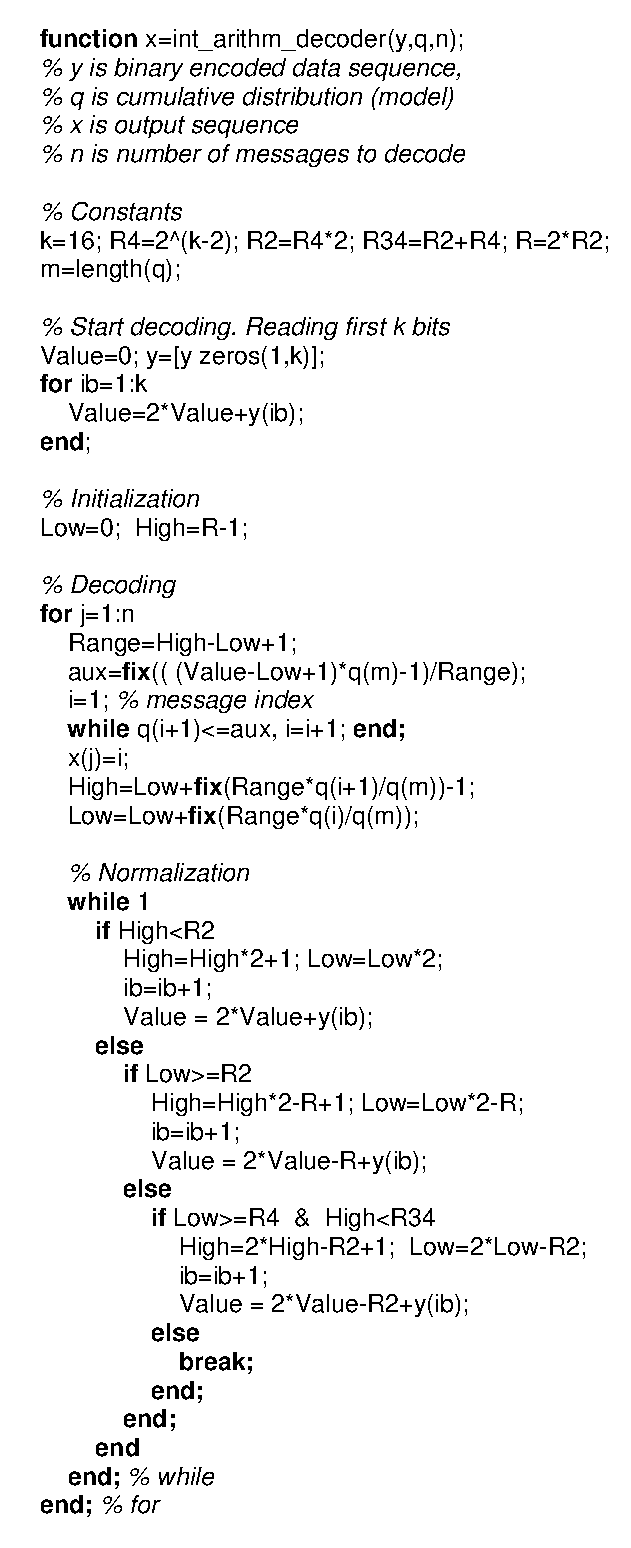
\includegraphics[width=0.28\textwidth]{fig_ar_decoder.eps}
  
  \end{multicols}
\end{frame}



\end{document} 